\documentclass[12pt,ngerman]{scrartcl}
\usepackage{tikz}
\usetikzlibrary{positioning}

\begin{document}

\begin{center}
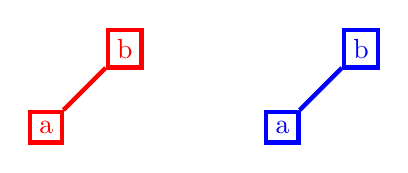
\begin{tikzpicture}[ultra thick]
  \begin{scope}[red]
 \node[draw, rectangle] (a) at (1,1){a};
 \node[draw, rectangle] (b) at (2,2){b};
 \draw(a) -- (b);
  \end{scope}
% gleiche Koordinaten wie oben, nur andere Farbe und xshift Transformation
  \begin{scope}[xshift=3cm,blue]
 \node[draw, rectangle] (a) at (1,1){a};
 \node[draw, rectangle] (b) at (2,2){b};
 \draw(a) -- (b);
  \end{scope}
\end{tikzpicture}
\end{center}

\end{document}


Google Gemini Erklärung:

tikz scopes are a powerful tool in LaTeX's TikZ package for creating nested environments within a TikZ picture. They allow you to define specific drawing areas with their own coordinate system, style settings, and transformations. This makes it easier to organize complex drawings and reuse elements.

Key features and benefits of tikz scopes:

 *   Nested environments: Scopes can be nested within each other, enabling hierarchical structures and modular design.
*    Custom coordinate systems: Each scope can have its own coordinate system, independent of the parent scope. This is useful for creating specific regions or subplots.
*    Style settings: Styles can be defined and applied within scopes, allowing you to customize the appearance of elements within the scope.
 *   Transformations: Transformations like scaling, rotation, and shifting can be applied to elements within a scope without affecting the rest of the picture.
* Reusability: Scopes can be defined as reusable macros, making it easier to create consistent elements and reduce code duplication.